\chapter{User Study}
\label{ch:Evaluation}

We hypothesized identifying important commits automatically and providing integrated access between commit and issue information could help a developer more effectively access the rationale for code.
To evaluate our hypothesis, we conducted a user study in the form of a semi-structured interview and targeted the following research questions:

\begin{itemize}[leftmargin=*]
    \item[] \label{itm:RQ1} \textbf{Research Question 1 (\entity{RQ1}):} \textit{Does highlighting important commits help software developers explore a file’s revision history more effectively?}
    \item[] \label{itm:RQ2} \textbf{Research Question 2 (\entity{RQ2}):} \textit{Does highlighting important commits help software developers explore a file’s revision history more efficiently?}
    \item[] \label{itm:RQ3} \textbf{Research Question 3 (\entity{RQ3}):} \textit{How useful is direct integration of issue information in the IDE for helping a developer search for code rationale information?}
  \end{itemize}

We describe our methodology designed to address these research questions in \autoref{sec:Method} and answer the research questions using the results of the evaluation in \autoref{sec:Results}.
We discuss the threats to validity of our evaluation in \autoref{sec:Threads-to-Validity}.

%%%%%%%%%%%%%%%%%%%%%%%%%%%%%%%%%%%%%%%%%%%%%%%%%%%%%%%%%%%%%%%%%%%%%%
\section{Method}
\label{sec:Method}

We designed the user study as an explorative, semi-structured interview composed of two parts with an estimated duration of 1 to 1.5 hours.
A semi-structured interview format allows us to maintain a focused discussion while also eliciting interesting responses and reasoning from participants \cite{shull_guide_2007}.
The semi-structured interview format is also appropriate as we seek to understand how participants interact with the commit history for a file and the Intelligent History plugin.
The study involved having participants explore the commit history of two Java classes from the Apache Kafka project to find answers to questions related to motivation and rationale behind changes in the classes.
The briefing for the study and the setup instructions can be found in Appendix \ref{sec:Briefing-and-Setup}.
We expected the participants to interact with commit and issue information found in the commit history in order to be able to answer these questions.

The first part of the user study session consisted of asking questions from two sets of questions about the motivation behind certain changes and aspects about specific Java classes from Apache Kafka.
These questions are presented in \autoref{tab:Question-Sets} and require exploring and locating particular commits in a given Java class' commit history to try to find code rationale information through inspecting the commits' full commit messages,
diffs, and any relevant Jira issues.
For each answer the participant provides to a question, the participant must justify their answer by referencing a combination of source code changes from diffs,
commit messages, and Jira issues from the Apache Kafka project.

In cases where a Jira issue referenced a Kafka Improvement Proposal (\entity{KIP}), we allowed the participant to visit these \entity{KIP}s in the browser.
Each question set pertains to a different Java class from the Apache Kafka project.
This facilitated an experiment where the participant would complete an initial set of questions without being allowed to use the features of Intelligent History plugin.
After completing the initial provided set of questions, the participant is introduced to the features of the Intelligent History plugin and permitted to use them to help them answer the second set of questions.
As shown in \autoref{tab:Question-Sets}, set A asks questions regarding the motivation behind particular changes in \class{Toplogy}, while set B asks the participant to identify potentially important or meaningful commits from the history and about motivation behind a specific method in \class{StreamsBuilder}.
The \class{Topology} class contains 22 commits and the \class{StreamsBuilder} class contains 45 commits respectively.
We limited the number of questions per class based on the number of commits in each class' commit history and to accomodate participants' varying preferences for and familiarity with exploring commit history in general.

The participants answered each question verbally to the author, who served as an observer and interviewer for each participant's session.
Upon sufficient answering of a question, the observer would provide the next question.
The criteria for sufficient answer was based on the participant's ability to provide a justification to their answer through referencing relevant parts of the source code, commits, and Jira issues.
Participants were permitted to think aloud and were also prompted by the observer who would occassionally ask the participant about their approach to how would they find the information to answer the question.

We divided the 10 participants into two groups of five participants such that one group received and completed set A first \emph{without} using the Intelligent History plugin, and set B afterwards \emph{with} introduction to the plugin and its features.
The other group received set B first to complete \emph{without} the plugin, and set A to complete \emph{with} permitted use of the plugin.
We swapped the order of the question sets for each group to study the performance of Intelligent History in assisting participants with answering questions from the different question sets.
There is overlap between the sets, specifically with questions A2 and B2 from \autoref{tab:Question-Sets}.
However, we anticipated the features of Intelligent History to provide the most utility to participants that receive set B as the question set they will be allowed to use Intelligent History for.
Question B1 from \autoref{tab:Question-Sets} expects the participant to examine the diffs, messages, and Jira issue for each commit in order to identify two changes that they can justify have a certain intent, which is to improve some functionality in \class{StreamsBuilder}. 

\begin{table}[h]
  \caption{
    The question sets used in the user study. 
    Set A pertains to the \class{Topology} class and set B relates to the \class{StreamsBuilder} class.
  }
  \centering
  \begin{tabular}{@{}ccl@{}}
  \toprule
  Set                                      & Class Name                                                   & \multicolumn{1}{c}{Question}                                                                                                                                                                                                                                                                                                                                            \\ \midrule
  \multicolumn{1}{|c|}{\multirow{3}{*}{A}} & \multicolumn{1}{c|}{\multirow{2}{*}{\class{Topology}}}       & \multicolumn{1}{p{8cm}|}{\begin{tabular}[c]{@{}p{8cm}}\small A1. Can you describe the motivation behind why the code segment on lines 717 to 722 was introduced and the benefit to the user of the Kafka \entity{API}?\end{tabular}}                                                                                                                                                             \\ \cmidrule(l){3-3} 
  \multicolumn{1}{|c|}{}                   & \multicolumn{1}{c|}{}                                        & \multicolumn{1}{p{8cm}|}{\begin{tabular}[c]{@{}p{8cm}}\small A2. There are several overloaded methods called \code{addSink} in this class. Can you describe in what context were these overloaded methods introduced to this class?\end{tabular}}                                                                                                                                             \\ \cmidrule(l){3-3} 
  \multicolumn{1}{|c|}{\multirow{2}{*}{B}} & \multicolumn{1}{c|}{\multirow{2}{*}{\class{StreamsBuilder}}} & \multicolumn{1}{p{8cm}|}{\begin{tabular}[c]{@{}p{8cm}}\small A1. Can you find two commits that introduced changes to improve some functionality in this class and justify why you chose them? The changes can not be cosmetic such as removing repeated words, removing deprecated code, or adding/modifying/removing documentation and comments.\end{tabular}} \\ \cmidrule(l){3-3} 
  \multicolumn{1}{|c|}{}                   & \multicolumn{1}{c|}{}                                        & \multicolumn{1}{p{8cm}|}{\small A2. Why is the \code{build} method in this class overloaded? Specifically, why was the overloaded build method in lines 623 to 630 introduced?}                                                                                                                                                                                                                \\ \bottomrule
  \end{tabular}
  \label{tab:Question-Sets}
\end{table}

The second part of the session consisted of asking a series of open-ended interview questions to gather information about the participant's background with respect to software development and experience in examining commits and issues from an issue tracking system (\entity{ITS}).
We also asked participants to compare their experience in completing the question sets without and with the use of Intelligent History.
The interview questions are available at Appendix \ref{sec:Interview-Questions}.
As part of the semi-structured format of the study, we would ask follow-up questions based on the participant's responses for further clarification and to probe further about unexpected responses. 
For example, if the participant stated they had little experience with working in a project that used an issue tracking system (\entity{ITS}), we would ask the participant about how they typically find and obtain code rationale information.

The interview sessions took place virtually over Zoom, where participants were asked to share their screen.
We recorded all of the sessions for manual review and documented each session with a summary.

\subsection{Participants}

We recruited 10 participants through public posting on social media and circulating a letter of initial contact within the author's professional network.
We focused on recruiting software developers with at least 1 year of experience in software development, which could include non-professional and professional experience.
Participants were compensated with entrance to a raffle for 1 of 5 Amazon gift cards valued at $\$40$ \entity{CAD}.
\autoref{tab:Participants} shows the demographic information we collected for each participant and which question set from \autoref{tab:Question-Sets} that the participant received first and second.
The participant is always introduced to the features of the Intelligent History plugin after completing the first of questions and is permitted to use the plugin features for the second set of questions.
The role for each participant indicates their occupation title at the time of the user study.
We generalized the participants' roles to ensure their anonymity.
Among 10 participants, 4 were students and 6 were full-time developers or engineers.
In terms of the participants' total years of experience in software development, the mean was 5.2 years and the median was 4.3 years.

\begin{table}[h]
  \caption{
    Participants by pseudo-initial, total years of experience (YoE) with separation by professional (p) and non-professional (n-p) experience, current role, and the question set the participant received first and second.
  }
  \centering
  \begin{tabular}{@{}c|clcc@{}}
  \toprule
  \multicolumn{1}{l}{Pseudo-initial} & \multicolumn{1}{l}{YoE (p/n-p)} & \multicolumn{1}{c}{Role} & \multicolumn{1}{l}{First Set} & \multicolumn{1}{l}{Second Set} \\ \midrule
  A                                  & 4.0 (1.0/3.0)                   & Firmware Developer       & A                             & B                               \\
  B                                  & 3.0 (2.8/0.2)                   & Software Developer       & B                             & A                               \\
  C                                  & 6.0 (3.0/3.0)                   & UX Engineer              & A                             & B                               \\
  D                                  & 4.5 (2.5/2.0)                   & Software Developer       & B                             & A                               \\
  E                                  & 13.0 (6.0/7.0)                  & Graduate Student         & A                             & B                               \\
  F                                  & 6.0 (2.0/4.0)                   & Software Developer       & B                             & A                               \\
  G                                  & 2.0 (0.0/2.0)                   & Undergraduate Student    & A                             & B                               \\
  H                                  & 3.5 (1.5/2.0)                   & Software Developer       & B                             & A                               \\
  I                                  & 4.0 (3.0/1.0)                   & Graduate Student         & A                             & B                               \\
  J                                  & 6.0 (2.0/4.0)                   & Graduate Student         & B                             & A                               \\ \bottomrule
  \end{tabular}
  \label{tab:Participants}
\end{table}

\subsection{Analysis}
\label{subsec:Analysis}

For quantitative analysis, we instrumented Intelligent History to log timestamps and events occuring within the IDE.
We logged the commits a participant examined for each question and the actions of Intelligent History that the participant invoked,
including the toggling of \textit{Highlight Important Changes} and the invocation of \textit{Show Diff Metadata} and \textit{Show Jira Metadata}.
This allows us to record the number of commits a participant investigated to answer a question and how the participant interacted with the Intelligent History plugin for answering the question set in which they were permitted to use its features.
We would also be able to trace which specific commits a participant examined as part of their search and if a commit was or would have been highlighted by Intelligent History.
From the quantitative metrics, we record the proportion of commits from a file's commit history that a participant examined to answer each question.
For each question a participant answers, we also record the proportion of a participant's examined commits that are highlighted commits according to Intelligent History,
the number of application switches a user makes between the \entity{IDE} and their browser for viewing Jira issues,
and the number of Jira issues that a participant viewed or accessed.
For the question set in which the participant was permitted to use Intelligent History, we consider the invocation of the \textit{Show Jira Metadata} feature as viewing a Jira issue
as the content of the issue is accessed from within the \entity{IDE}.

After obtaining the quantitative data, we conduct a single-tailed, two-sample $t$-test to test for statistically significant difference between the proportion of commits from the commit history examined by the group of participants that completed a question set \emph{without} Intelligent History and the group of participants that completed the same question set \emph{with} Intelligent History.
We use the null hypothesis ($H_{0}$): 
\textit{The mean proportion of commits from a commit history examined by the group without Intelligent History and the group with Intelligent History are equal.}
For each question asked in the user study, we compute the $t$-value and $p$-value for the group that completed the question \emph{without} Intelligent History and the group that completed the question \emph{with} Intelligent History.
For the significance level $\alpha = 0.05$, we reject the null hypothesis if $p < 0.05$.
We performed this $t$-test for each question and compared the group who completed the question without Intelligent History and the group who completed with Intelligent History.
Each group contains 5 samples, hence the degrees of freedom for each $t$-test is $df = 8$.

For qualitative analysis, we used the session recordings and logs to construct directed graphs for each participant's session to visualize how they explored commit history to answer the question sets and the impact of Intelligent History on their exploration.
We regard these graphs as commit history exploration graphs and constructed a set of these graphs for each participant, one for each question the participant worked on.
Nodes in the graph are represented by commit hashes and Jira issue IDs while edges express the participant's movement from examining one commit to another.
Bold commit hashes indicate commits that would be highlighted by Intelligent History, while light hashes indicate non-highlighted commits.
Italicized commit hashes are those for which the participant was heard reading or skimming the commit message subject aloud but did not investigate further by explicitly selecting the commit for further viewing.
We use a green checkmark to signal when a participant provided an answer to the question and a globe icon to show when a participant has made an application switch between the \entity{IDE} and their browser to further examine a Jira issue.

To analyze the participants' responses to the open-ended interview questions, we create a set of flowcharts to illustrate the relationship between the participant's experience with looking at issues and commits,
the commit history exploration approach they exhibitied when searching for the answers to the question sets, and the features of Intelligent History they expressed the most enthusiasm for.
We determined a participant's commit history exploration approach based on the structure of the commit history graphs we produced for each participant.
Each participant tended to use the same commit history exploration strategy throughout the study, irrespective of the nature of the question asked and the presence of Intelligent History.

%%%%%%%%%%%%%%%%%%%%%%%%%%%%%%%%%%%%%%%%%%%%%%%%%%%%%%%%%%%%%%%%%%%%%%
\section{Results}
\label{sec:Results}

We summarize the quantitative results collected through logs and screen recordings in \autoref{tab:Results-Quantitative-AB} for participants who received question set A first, then B.
Similarly, the results for participants who received question B, then A are shown in \autoref{tab:Results-Quantitative-BA}.
As stated in \autoref{sec:Method}, set A corresponds to the \class{Topology} class, which contains 22 commits in its commit history, 
while set B corresponds to the \class{StreamsBuilder} class, which contains 45 commits in its commit history.
Overall, participants who did not use Intelligent History examined a higher mean proportion of commits to answer both questions A1, A2, and B1.

The results of the $t$-tests for determining significant statistical differences in the mean proportion of commits are summarized in \autoref{tab:t-test}.
For questions A1 and B2, we fail to reject the null hypothesis, which states that the mean proportion of commits examined by the group without Intelligent History and the group with Intelligent History are equal.
However, for questions A2 and B1, we reject the null hypothesis, indicating the mean proportion of commits examined by the group without Intelligent History and the group without Intelligent History are not equal.
Thus, there is a significant difference in the mean proportion of commits examined between the group that does not use Intelligent History and the group that does use Intelligent History to answer questions A(b) and B(a).

\begin{table}[h]
  \caption{
    Results of single-tailed, two-sample $t$-tests at $\alpha = 0.05$ and $df = 8$ to determine if there is a significant difference between the proportion of commits examined from a commit history
    with and without Intelligent History.
  }
  \centering
  \begin{tabular}{@{}ccccc@{}}
    \toprule
    Set                                     & Question               & \multicolumn{1}{c}{$t$-value} & \multicolumn{1}{c}{$p$-value} & $H_{0}$ \\ \midrule
    \multicolumn{1}{c|}{\multirow{2}{*}{A}} & \multicolumn{1}{c|}{A1} & 1.53                        & 0.08                        & Fail to reject   \\ \cmidrule(l){2-5} 
    \multicolumn{1}{c|}{}                   & \multicolumn{1}{c|}{A2} & 2.13                        & 0.03                        & Reject   \\ \midrule
    \multicolumn{1}{c|}{\multirow{2}{*}{B}} & \multicolumn{1}{c|}{B1} & 2.37                        & 0.02                        & Reject   \\ \cmidrule(l){2-5} 
    \multicolumn{1}{c|}{}                   & \multicolumn{1}{c|}{B2} & -0.66                       & 0.26                        & Fail to reject   \\ \bottomrule
  \end{tabular}
  \label{tab:t-test}
\end{table}

We described constructing commit history exploration graphs in \autoref{subsec:Analysis}. 
A sample of two commit history exploration graph we constructed to illustrate participants \participant{F} and \participant{H}’s exploration to answer question B1 from \autoref{tab:Question-Sets} is shown in \autoref{fig:Exploration-Graphs}.

\begin{figure}[h]
  \centering%
  \subfloat[\centering \participant{F}'s commit history exploration in answering question B1 \emph{without} Intelligent History. \label{subfig:Exploration-Graph-A}]{{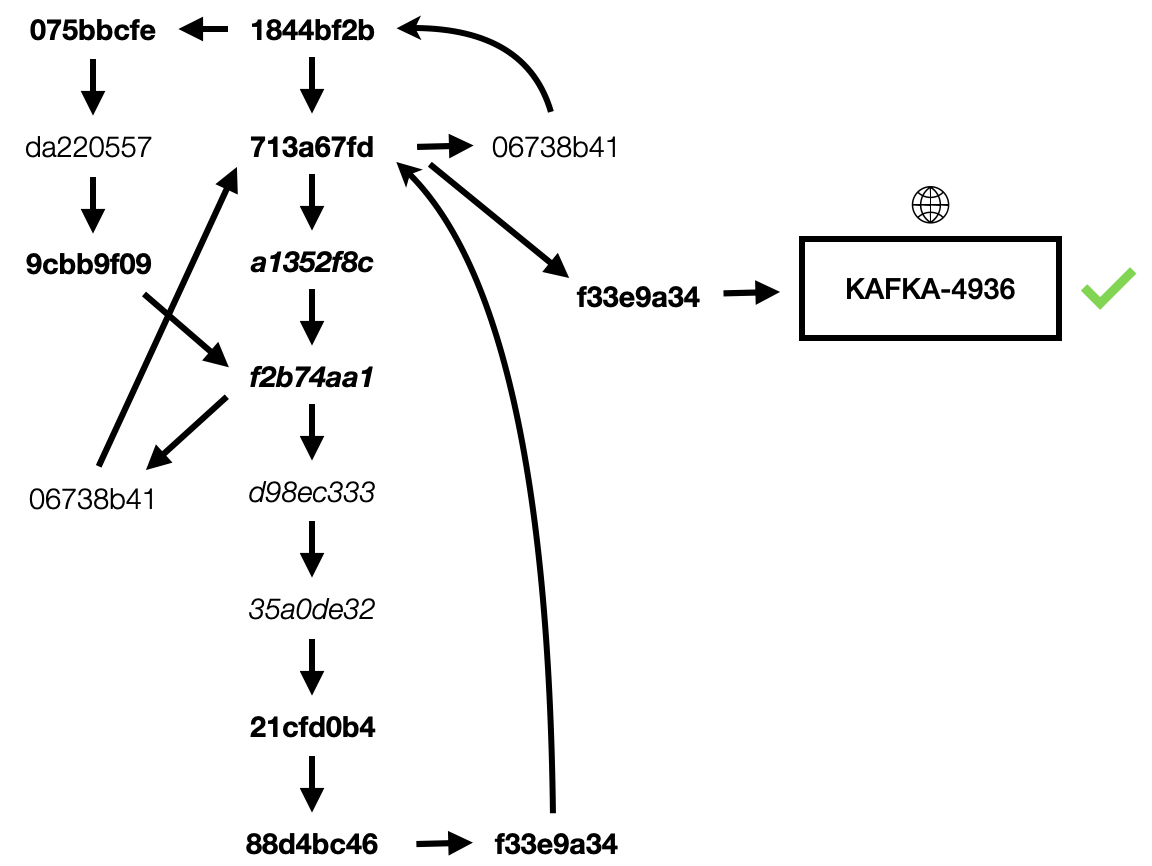
\includegraphics[width=5.5cm]{./images/graph-sample-A.png}}}%
  \qquad
  \subfloat[\centering \participant{H}'s commit history exploration in answering question B1 \emph{without} Intelligent History. \label{subfig:Exploration-Graph-B}]{{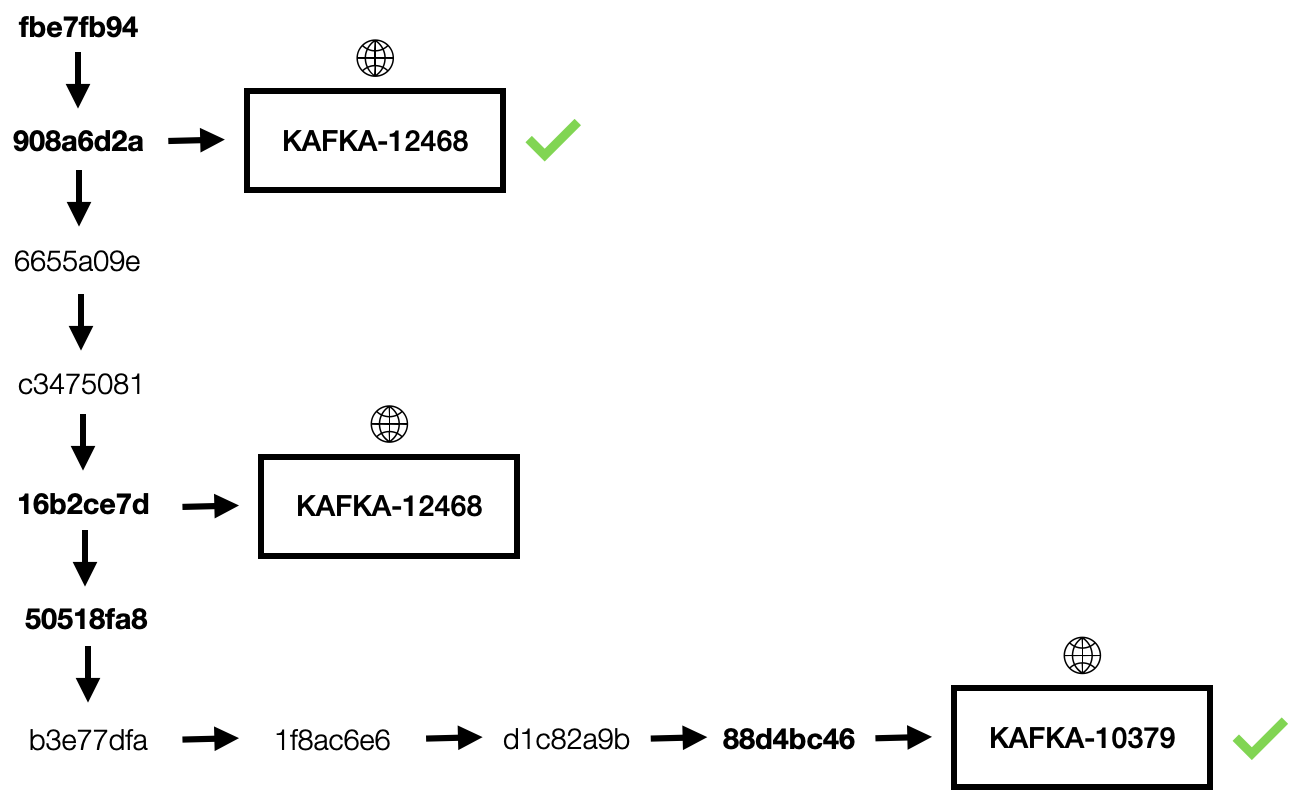
\includegraphics[width=5.5cm]{./images/graph-sample-B.png}}}%
  \caption{
    Commit history exploration graphs.
  }%
  \label{fig:Exploration-Graphs}%
\end{figure}

As a demonstration of how we devised themes for the participants' exhibited approaches for commit history exploration, \autoref{subfig:Exploration-Graph-A} illustrates the participant F's approach to finding two meaningful commits as per question B(a) without using Intelligent History.
The commit history exploration graph for \participant{F} shows they examined 19 out of 45 commits.
Participant \participant{F} began their search by scanning the commit message subjects to reduce their search and performed backtracking to review previously examined commits.
We characterize the structure of the graph for \participant{F} as cyclic with skimming.
Meanwhile, the commit history graph for \participant{H} shown in \autoref{subfig:Exploration-Graph-B}, who answered the same question without Intelligent History, shows they examined 10 out of 45 commits.
Participant \participant{H} exhibited an approach where they examined each commit sequentially in chronological order.
We characterize the structure of the graph for \participant{H} and their commit history exploration approach as linear to describe the participant's sequential or chronological exploration of the commit history.

The flowchart showing the relationship between each participant's background related to looking at commits and issues,
the commit history exploration approach they used, and their preferred features provided by Intelligent History is displayed in \autoref{fig:Flow-Chart-Individual}.
The features of Intelligent History are the actions we detailed in \autoref{sec:Implementation}, which are 
(A) \textit{Highlight Important Changes}; (B) \textit{Show Diff Metadata}; and (C) textit{Show Jira Metadata}.
We also present an aggregated version as a Sankey diagram in \autoref{fig:Flow-Chart-Aggregate} and a tabular form in \autoref{tab:Flow-Chart-Tabular} for clarity.

\begin{figure}[h]
  \centering
  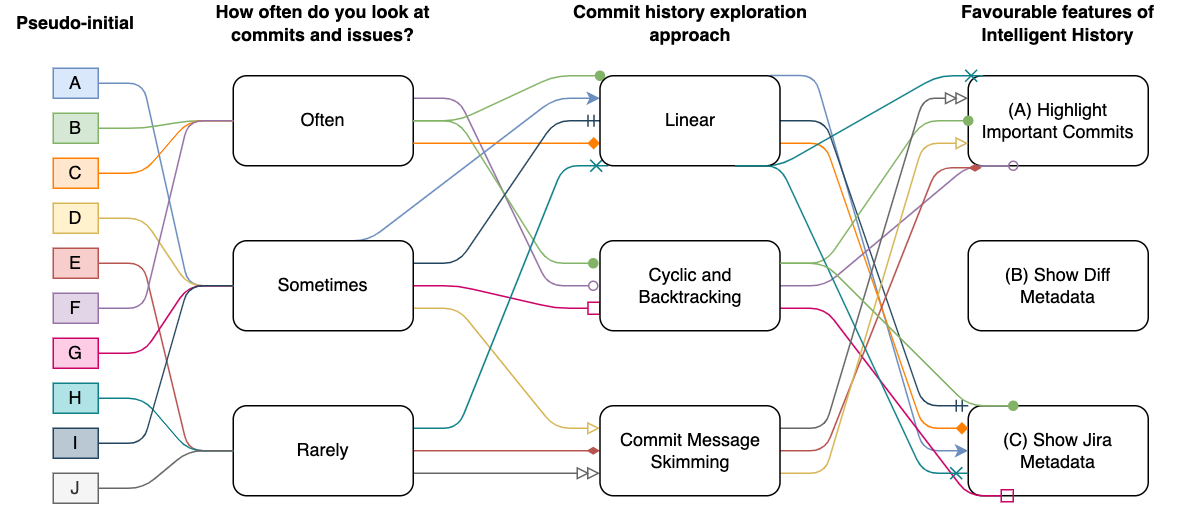
\includegraphics[width=12cm]{./images/flow-chart-ind.png}
  \caption{
    The relationship between how often a participant looks at commits and issues, the approach they exhibited to exploring commit history overall, and the features of Intelligent History they showed the most enthusiasm for.
  }
  \label{fig:Flow-Chart-Individual}
\end{figure}

\begin{figure}[h]
  \centering
  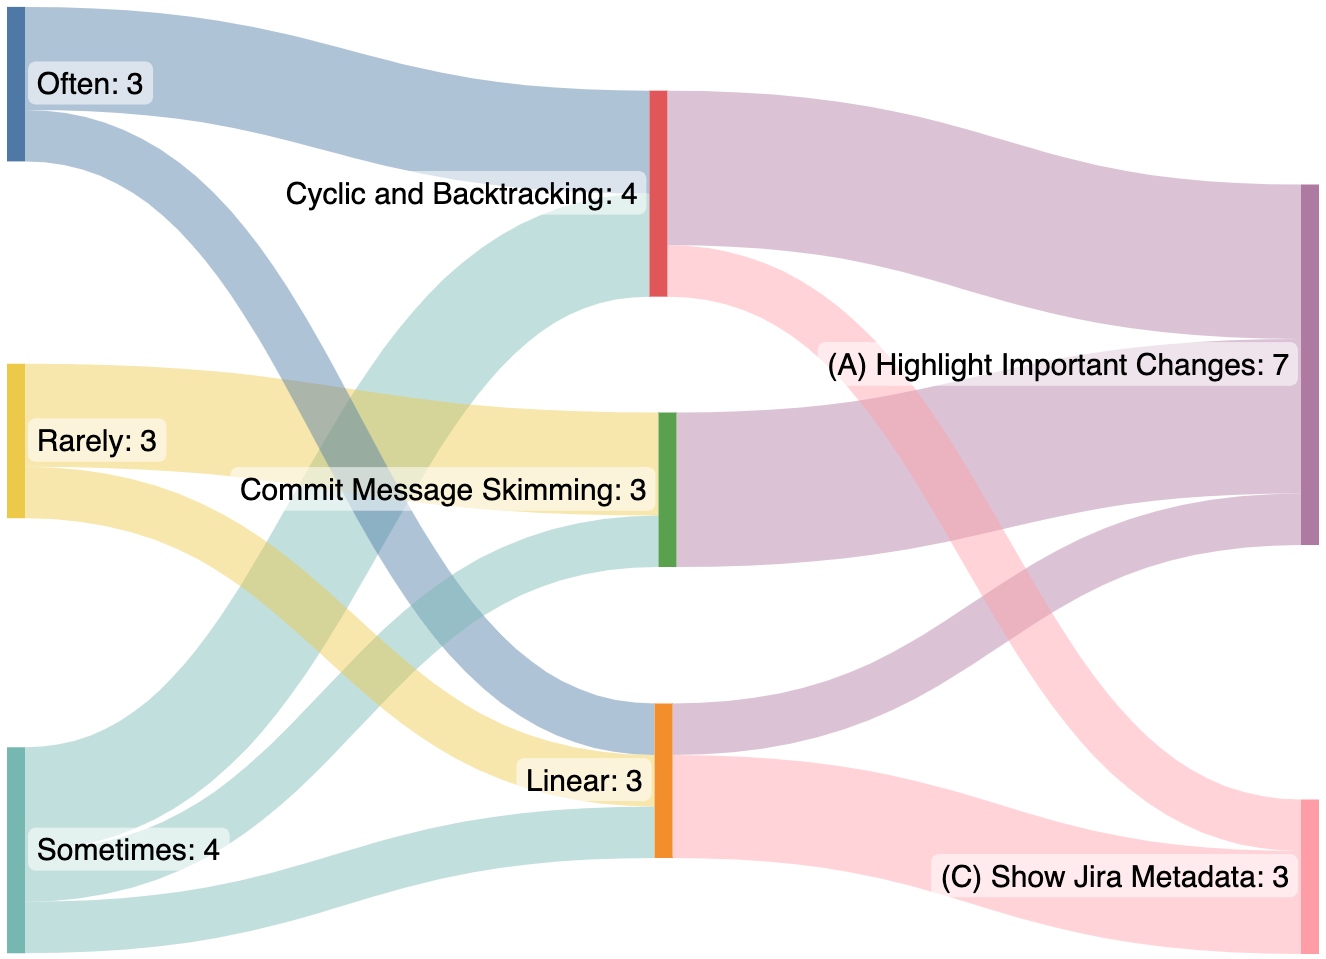
\includegraphics[width=10cm]{./images/flow-chart-aggr.png}
  \caption{
    Sankey diagram to represent the information in \autoref{fig:Flow-Chart-Individual} and \autoref{tab:Flow-Chart-Tabular}
  }
  \label{fig:Flow-Chart-Aggregate}
\end{figure}

The majority of participants, 6 out of 10, preferred feature (A) from Intelligent History the most,
whereas the other 4 participants preferred feature (C).
Notably, all 5 of the participants who received question set A to answer with Intelligent History responded most positively to commit history highlighting as a feature, 
whereas 4 out of the 5 participants who received question set B to answer with Intelligent History responded most positively to gaining quick access to Jira issue information within the \entity{IDE} as a feature.
This indicates some level of correlation between the question set and the participants' most preferred features of Intelligent History.

None of the participants chose feature (B), though this was anticipated as this feature was provided to give the user context as to how Intelligent History highlights commits in feature (A).
Of the 3 participants who often look at commits and issues, none demonstrated commit message skimming as a strategy for exploring commit history.
Similarly, of the 3 participants who rarely look at commits and issues, none employ an commit history exploration approach that could be described as cyclic and backtracking.
There does not appear to be any concrete associations between the background of a participant with regard to looking at commits and issues,
their exhibited approach to exploring commit history, and the feature of Intelligent History they had a strong preference for.

\begin{landscape}
  \begin{figure}
    \footnotesize
    \caption{
      A tabular form of \autoref{fig:Flow-Chart-Individual}.
    }
    \centering
    \begin{tabular}{@{}c|ccc@{}}
      \toprule
      \textbf{Pseudo-initial} & \textbf{\begin{tabular}[c]{@{}c@{}}How often do you look\\ at commits and issues?\end{tabular}} & \textbf{\begin{tabular}[c]{@{}c@{}}Commit history\\ exploration approach\end{tabular}} & \textbf{\begin{tabular}[c]{@{}c@{}}Favourable features of\\ Intelligent History\end{tabular}} \\ \midrule
      A                       & Sometimes                                                                                       & Cyclic and Backtracking                                                                & (C) Show Jira Metadata                                                                        \\ \midrule
      B                       & Often                                                                                           & Cyclic and Backtracking                                                                & (A) Highlight Important Changes                                                               \\ \midrule
      C                       & Often                                                                                           & Linear                                                                                 & (C) Show Jira Metadata                                                                        \\ \midrule
      D                       & Sometimes                                                                                       & Commit Message Skimming                                                                & (A) Highlight Important Changes                                                               \\ \midrule
      E                       & Rarely                                                                                          & Commit Message Skimming                                                                & (A) Highlight Important Changes                                                               \\ \midrule
      F                       & Often                                                                                           & Cyclic and Backtracking                                                                & (A) Highlight Important Changes                                                               \\ \midrule
      G                       & Sometimes                                                                                       & Cyclic and Backtracking                                                                & (C) Show Jira Metadata                                                                        \\ \midrule
      H                       & Rarely                                                                                          & Linear                                                                                 & (A) Highlight Important Changes                                                               \\ \midrule
      I                       & Sometimes                                                                                       & Linear                                                                                 & (C) Show Jira Metadata                                                                        \\ \midrule
      J                       & Rarely                                                                                          & Commit Message Skimming                                                                & (A) Highlight Important Changes                                                               \\ \bottomrule
    \end{tabular}
    \label{tab:Flow-Chart-Tabular}
  \end{figure}
\end{landscape}

%% BEGIN: Large landscape tables
\begin{landscape}
  \begin{table}
    \footnotesize
    \caption{
      Summary of results for participants who received question set A first to complete without the plugin and question set B after to complete with the plugin.
      For each question set and question, the table shows the percentage of commits from the commit history that the participant examined (\%CE), 
      the percentage of the participant's examined commits that would be or were highlighted by the plugin (\%HC),
      the number of application switches between the \entity{IDE} and the browser (\#AC) that the participant made,
      and the number of Jira issues the participant viewed or accessed (\#IV).
    }
    \centering
    \begin{tabular}{@{}ccccccccccccccccc@{}}
      \toprule
      \multicolumn{1}{l}{}                & \multicolumn{8}{c}{Set A (without plugin)}                                                                                                                            & \multicolumn{8}{c}{Set B (with plugin)}                                                                                                                                                                 \\ \midrule
      \multicolumn{1}{c|}{}               & \multicolumn{4}{c|}{A1}                                  & \multicolumn{4}{c|}{A2}                                                                                    & \multicolumn{4}{c|}{B1}                                                                     & \multicolumn{4}{c}{B2}                                                                                    \\ \midrule
      \multicolumn{1}{c|}{Pseudo-initial} & \%CE      & \%HC      & \#AS & \multicolumn{1}{l|}{\#IV} & \multicolumn{1}{l}{\%CE} & \multicolumn{1}{l}{\%HC} & \multicolumn{1}{l}{\#AS} & \multicolumn{1}{l|}{\#IV} & \%CE      & \multicolumn{1}{l}{\%HC} & \multicolumn{1}{l}{\#AS} & \multicolumn{1}{l|}{\#IV} & \multicolumn{1}{l}{\%CE} & \multicolumn{1}{l}{\%HC} & \multicolumn{1}{l}{\#AS} & \multicolumn{1}{l}{\#IV} \\ \midrule
      \multicolumn{1}{c|}{A}              & 40.9 (9)  & 55.6 (5)  & 1    & \multicolumn{1}{c|}{1}    & 27.3 (6)                 & 83.3 (5)                 & 1                        & \multicolumn{1}{c|}{1}    & 15.6 (7)  & 100.0 (7)                & 0                        & \multicolumn{1}{c|}{4}    & 6.7 (3)                  & 100.0 (3)                & 0                        & 1                        \\
      \multicolumn{1}{c|}{C}              & 4.5 (1)   & 100.0 (1) & 1    & \multicolumn{1}{c|}{1}    & 27.3 (6)                 & 83.3 (5)                 & 1                        & \multicolumn{1}{c|}{1}    & 6.7 (3)   & 100.0 (3)                & 0                        & \multicolumn{1}{c|}{2}    & 0.0 (0)                  & N/A                      & 0                        & 0                        \\
      \multicolumn{1}{c|}{E}              & 36.3 (8)  & 62.5 (5)  & 1    & \multicolumn{1}{c|}{1}    & 68.1 (15)                & 66.7 (10)                & 1                        & \multicolumn{1}{c|}{1}    & 35.6 (16) & 100.0 (16)               & 1                        & \multicolumn{1}{c|}{3}    & 8.9 (4)                  & 100.0 (4)                & 0                        & 1                        \\
      \multicolumn{1}{c|}{G}              & 86.3 (19) & 57.9 (11) & 1    & \multicolumn{1}{c|}{1}    & 36.3 (8)                 & 75.0 (6)                 & 1                        & \multicolumn{1}{c|}{1}    & 13.3 (6)  & 100.0 (6)                & 3                        & \multicolumn{1}{c|}{5}    & 6.7 (3)                  & 100.0 (3)                & 1                        & 2                        \\
      \multicolumn{1}{c|}{I}              & 4.5 (1)   & 83.3 (5)  & 1    & \multicolumn{1}{c|}{1}    & 36.3 (8)                 & 75.0 (6)                 & 1                        & \multicolumn{1}{c|}{1}    & 6.7 (3)   & 100.0 (3)                & 0                        & \multicolumn{1}{c|}{2}    & 6.7 (3)                  & 100.0 (3)                & 0                        & 1                        \\ \midrule
      \multicolumn{1}{l|}{Mean}           & 34.5      & 68.5      & 1    & \multicolumn{1}{c|}{1}    & 39.1                     & 76.7                     & 1                        & \multicolumn{1}{c|}{1}    & 15.6      & 100.0                    & 0.8                      & \multicolumn{1}{c|}{3.2}  & 5.8                      & 100.0                    & 0.2                      & 1                        \\
      \multicolumn{1}{l|}{Median}         & 36.3      & 62.5      & 1    & \multicolumn{1}{c|}{1}    & 36.3                     & 75.0                     & 1                        & \multicolumn{1}{c|}{1}    & 13.3      & 100.0                    & 0.0                      & \multicolumn{1}{c|}{3.0}  & 6.7                      & 100.0                    & 0.0                      & 1                        \\ \bottomrule
    \end{tabular}
    \label{tab:Results-Quantitative-AB}
  \end{table}
\end{landscape}

\begin{landscape}
  \begin{table}
    \footnotesize
    \caption{
      Summary of results for participants who received question set B first to complete without the plugin and question set A after to complete with permitted use of the plugin.
      The same columns as shown in \autoref{tab:Results-Quantitative-AB} are used.
    }
    \centering
    \begin{tabular}{@{}ccccccccccccccccc@{}}
      \toprule
      \multicolumn{1}{l}{}                & \multicolumn{8}{c}{Set A (with plugin)}                                                                                                                              & \multicolumn{8}{c}{Set B (without plugin)}                                                                                                                                                              \\ \midrule
      \multicolumn{1}{c|}{}               & \multicolumn{4}{c|}{A1}                                 & \multicolumn{4}{c|}{A2}                                                                                    & \multicolumn{4}{c|}{B1}                                                                     & \multicolumn{4}{c}{B2}                                                                                    \\ \midrule
      \multicolumn{1}{c|}{Pseudo-initial} & \%CE     & \%HC      & \#AS & \multicolumn{1}{l|}{\#IV} & \multicolumn{1}{l}{\%CE} & \multicolumn{1}{l}{\%HC} & \multicolumn{1}{l}{\#AS} & \multicolumn{1}{l|}{\#IV} & \%CE      & \multicolumn{1}{l}{\%HC} & \multicolumn{1}{l}{\#AS} & \multicolumn{1}{l|}{\#IV} & \multicolumn{1}{l}{\%CE} & \multicolumn{1}{l}{\%HC} & \multicolumn{1}{l}{\#AS} & \multicolumn{1}{l}{\#IV} \\ \midrule
      \multicolumn{1}{c|}{B}              & 4.5 (1)  & 100.0 (1) & 1    & \multicolumn{1}{c|}{1}    & 9.0 (2)                  & 100.0 (2)                & 0                        & \multicolumn{1}{c|}{1}    & 35.6 (16) & 37.5 (6)                 & 2                        & \multicolumn{1}{c|}{2}    & 4.4 (2)                  & 100.0 (1)                & 0                        & 0                        \\
      \multicolumn{1}{c|}{D}              & 31.8 (7) & 100.0 (1) & 1    & \multicolumn{1}{c|}{1}    & 13.3 (6)                 & 100.0 (1)                & 1                        & \multicolumn{1}{c|}{1}    & 20.0 (9)  & 55.6 (5)                 & 2                        & \multicolumn{1}{c|}{2}    & 8.9 (4)                  & 100.0 (4)                & 2                        & 2                        \\
      \multicolumn{1}{c|}{F}              & 4.5 (1)  & 100.0 (1) & 1    & \multicolumn{1}{c|}{1}    & 13.6 (3)                 & 100.0 (3)                & 1                        & \multicolumn{1}{c|}{1}    & 42.2 (19) & 42.1 (8)                 & 1                        & \multicolumn{1}{c|}{1}    & 2.2 (1)                  & 100.0 (1)                & 1                        & 1                        \\
      \multicolumn{1}{c|}{H}              & 4.5 (1)  & 100.0 (1) & 1    & \multicolumn{1}{c|}{1}    & 31.8 (7)                 & 85.7 (6)                 & 1                        & \multicolumn{1}{c|}{1}    & 22.2 (10) & 50.0 (5)                 & 3                        & \multicolumn{1}{c|}{3}    & 8.9 (4)                  & 100.0 (4)                & 1                        & 1                        \\
      \multicolumn{1}{c|}{J}              & 4.5 (1)  & 100.0 (1) & 1    & \multicolumn{1}{c|}{1}    & 31.8 (7)                 & 100.0 (7)                & 0                        & \multicolumn{1}{c|}{1}    & 46.7 (21) & 71.4 (15)                & 2                        & \multicolumn{1}{c|}{2}    & 6.7 (3)                  & 100.0 (3)                & 1                        & 1                        \\ \midrule
      \multicolumn{1}{l|}{Mean}           & 10.0     & 100.0     & 1    & \multicolumn{1}{c|}{1}    & 19.9                     & 97.1                     & 0.6                      & \multicolumn{1}{c|}{1}    & 33.3      & 51.3                     & 2                        & \multicolumn{1}{c|}{2}    & 6.2                      & 100.0                    & 1                        & 1                        \\
      \multicolumn{1}{l|}{Median}         & 4.5      & 100.0     & 1    & \multicolumn{1}{c|}{1}    & 13.6                     & 100.0                    & 1                        & \multicolumn{1}{c|}{1}    & 35.6      & 50.0                     & 2                        & \multicolumn{1}{c|}{2}    & 6.7                      & 100.0                    & 1                        & 1                        \\ \bottomrule
    \end{tabular}
    \label{tab:Results-Quantitative-BA}
  \end{table}
\end{landscape}
%% END: Large landscape tables

%%%%%%%%%%%%%%%%%%%%%%%%%%%%%%%%%%%%%%%%%%%%%%%%%%%%%%%%%%%%%%%%%%%%%%

\subsection{RQ1}
\label{subsec:RQ1}

\RQ{1}{Does highlighting important commits help software developers explore a file’s revision history more effectively?}
This research question is primarily concerned with the correctness of the participants' answers to the questions.

%%%%%%%%%%%%%%%%%%%%%%%%%%%%%%%%%%%%%%%%%%%%%%%%%%%%%%%%%%%%%%%%%%%%%%

\subsection{RQ2}
\label{subsec:RQ2}

\RQ{2}{Does highlighting important commits help software developers explore a file’s revision history more efficiently?}
We define efficient as the proportion of commits from a file's commit history that a developer must examine before obtaining the answer to questions about the intent behind code changes.
Under this definition, we could consider that commit history highlighting does help with efficiently exploring a file's commit history for questions related to identifying meaningful source changes and the rationale behind those changes when the developer must navigate a broad commit history for a file. 
This is evidenced by the participants who used Intelligent History to answer A2 and B1 as they examined a significantly smaller proportion of a given file's commit history to obtain the code ratianale information needed for answering the questions asked in the user study.

\begin{observation}
  Commit history highlighting can be efficient in helping software developers efficiently explore commit history for code rationale information by examining a smaller proportion of the commits in a file's commit history.
  In particular, commit history highlighting makes identifying and searching for meaningful source code changes across a broad commit history more efficient but has less impact when trying to find rationale information for specific code segments in a file.
\end{observation}

\subsubsection{Navigating a Broad Commit History}

For question A2, participants who used Intelligent History examined a mean of 19.9\% of the commit history for the \class{Topology} class,
while participants who did not use Intelligent History examined a mean of 39.1\% of the same commit history. 
Moreover, of the participants who used Intelligent History and the proportion of commits they examined,
a mean of 97.1\% of the commits they examined were highlighted commits.
For the group that did not use Intelligent History, a mean of 76.1\% of the commits they examined would have been highlighted commits under Intelligent History's \textit{Highlight Important Changes} feature.

To answer question A2, participants needed to find a commit that introduced further \newline 
\code{addSink} method overloads later in the commit history as participants were informed that the initial commit in the commit history for the \class{Topology} class introduced a set of overloaded \code{addSink} methods to begin with.
The specific commit which does this is commit \commitref{f33e9a34}{https://github.com/apache/kafka/commit/f33e9a346e22e29bb66e0ea0f3442903d136ca67} with the following commit message title:

\begin{center}
  \jira{KAFKA-4936:}{Add dynamic routing in Streams (\#5018)} 
\end{center}

Participants were not expected to be able to identify this commit based on its commit message title alone.
However, participants were prompted or intuited to locate a particular commit that introduced further overloads later in the history to understand why additional overloads were introduced to the \class{Topology} class.
This could be done through examining diffs of potentially interesting commits for commits that were made after the initial commit in the \class{StreamsBuilder} commit history.

Interestingly, all of the participants who used Intelligent History to answer A2 responded most positively to the \textit{Highlight Important Changes} feature of Intelligent History \participants{BDFHJ} (see \autoref{tab:Participants} and \autoref{tab:Flow-Chart-Tabular}).
Participants commented on the utility of commit history highlighting for focusing their attention on commits that were highlighted, ignoring non-highlighted commits which they regarded as ``irrelevant'' or ``minor'' \participants{BF}.
It may be worth noting that of these 5 participants, 2 employed a commit history exploration approach that could be described as cyclic and backtracking based on their commit history exploration graphs \participants{BF},
2 use commit message skimming \participants{DJ}, and 1 used a linear approach \participants{H}.
Specifically regarding answering A2, participant \participant{H} stated:

\begin{quote}
  [Highlighting commits] was amazing for speeding up what I had to search for. 
  Especially, in finding that sink issue [in A2], if I didn’t have the pencil [Highlight Important Changes feature], 
  I think I would have gone through all the commits backwards and just try to see what the diffs are 
  but it removed a bunch of the ones that it [Intelligent History] deemed not useful and it ended up being correct so I just skipped over a bunch [of commits].
\end{quote}

Comparing their experiences for answering the question set without and with Intelligent History, 
participants commented on the effect of commit history highlighting making commit history exploration faster by reducing the amount of irrelevant commits they would have examined \participants{DFHJ}.
Participant \participant{D} stated: ``\textit{[The highlighting] allowed for me to skim through the necessary commits a lot quicker \dots and visually reduces the amount of clutter I had to look at.}''

Meanwhile, in answering question B1, participants who used Intelligent History examined a mean of 15.6\% of the commit history for the \class{StreamsBuilder} class,
whereas participants who did not use Intelligent History examined a mean of 33.3\% of the same commit history.
Of the commits that the group who used Intelligent History examined for answering B1, a mean of 100.0\% of the commits were highlighted commits.
For the group who did not use Intelligent history to answer B1, a mean of 51.3\% of the commits they examined would have been highlighted commits if they used Intelligent History.

Question B1 necessitated for the participants to examine commits and diffs in the \class{StreamsBuilder} commit history to try to identify meaningful source code changes that were made to the class.
We clarified a meaningful source code change to be a commit that changes or improves some functionality or behaviour in the class and expected participants to utilize the diffs and intent of a change's author to justify their answer.
Despite the group of participants who used Intelligent History to answer B2 looking at less than half the proportion of commits that the group who did not use Intelligent History looked at (15.6\% compared to 33.3\%),
only 1 participant emphasized commit history highlighting as a feature that made the strongest impression on them \participants{E}, whereas the remaining 4 participants showed a preference for the \textit{Show Jira Metadata} feature of Intelligent History instead \participants{ACGI}.
Participant \participant{E} said:

\begin{quote}
  I think that the biggest benefit [of Intelligent History] was especially removing minor changes. 
  It’s really handy; it filters a bunch of -- not garbage -- but noise in the commit history. 
  With just this single feature [commit history highlighting], it’s already worth using the plugin.
\end{quote}

On the commit history highlighting feature, participant \participant{A} said:

\begin{quote}
  I liked the highlighting. 
  It’s nice to not look at so many commits. 
  [\dots] Looking at the history without the highlighting is kind of overwhelming because it’s just like ``oh my god, this is a flood of commits, what are we going to do?'' 
  but when you get rid of the less important ones, it’s [\dots] much more manageable.
\end{quote}

\subsubsection{Locating Rationale for a Code Fragment}

As captured from the results of the $t$-test in \autoref{tab:t-test}, there was less significant difference in the proportion of commits examined by the groups for answering questions A1 and B2.
Both questions A1 and B2 are similar in nature as they require the participant to inspect a specific section of code given by line numbers and attempt to locate commits relevant to these code segments.
Participants who vocalized familiarity with using \entity{git} ``blame'' were shown and permitted to use the native ``Show History for Selection'' feature in IntelliJ to narrow down the commits to look at.
This native feature enabled participants to view commits affecting selected fragments of source code.

In recognition of the suitability of commit history highlighting for certain types of questions,
2 participants who received question set B first without Intelligent History and received question set A after with Intelligent History commented on wishing to have been able to use Intelligent History's commit highlighting feature for question B1 instead as B1
required manual exploration of a large commit history \participants{BD}.
Participant \participant{B} mentioned:

\begin{quote}
  [For some of] the questions [I was] asked [\dots] the plugin didn’t help that much. 
  For example, one of the questions in the \class{StreamsBuilder} class was to look for commits that improve things, 
  so I feel like if I had to redo that task, then using the highlighting would have been useful.
\end{quote}

For question A1, 6 participants used the ``Show History for Selection'' feature \participants{CEFHIJ},
and the other 4 participants manually found the commit that introduced the change and contained the rationale information by reading the commit mesage subjects and using the chronological information based on other commit timestamps \participants{ABDG}.
For question B2, the failure to reject the null hypothesis may be attributed to the fact that the commit \commitref{e09d6d79}{https://github.com/apache/kafka/commit/e09d6d796f5a0b840519021d7f6435c65f88a60a} which contains the information necessary for answering this question has the message title: 

\begin{center}
  \jira{KAFKA-7027:}{Add overloaded build method to StreamsBuilder (\#5437)} 
\end{center}

Hence, participants used to using version control tools for similar questions encountered in every day work would be able to quickly narrow down the commit needed to answer the question without requiring traversal of the file's commit history.
Due to the nature of A1 and B2 and their answerability via other native features of IntelliJ, our samples may be insufficient for obtaining evidence to show a significant difference in commit history exploration efficiency between the group that does not use Intelligent History and the group that does use Intelligent History for questions that ask about specific sections of code from a Java class.
Thus, based on our analysis of A2 and B1, we make the observation that participants who use Intelligent History with its commit highlighting feature look at a smaller proportion of commits from a file's commit history when answering questions related to
identifying and finding meaningful source code changes over a broad commit history.
Participant \participant{A} expresses a beneficial use case of commit history highlighting for reducing the number commits a software developer examines:

\begin{quote}
  If I was trying to get a sense of major changes in a file, like say there was an issue that came up in a file and I’m looking for where it could have gotten introduced, 
  then that [highlighting commits] would be very useful because it gets rid of all the changes that don’t matter. 
\end{quote}

%%%%%%%%%%%%%%%%%%%%%%%%%%%%%%%%%%%%%%%%%%%%%%%%%%%%%%%%%%%%%%%%%%%%%%

\subsection{RQ3}
\label{subsec:RQ3}

\RQ{3}{How useful is direct integration of issue information in the IDE for helping a developer search for code rationale information?}

As mentioned in \autoref{subsec:RQ2} previously, 4 of the 5 participants who answered B1 using Intelligent History actually favoured the \textit{Show Jira Metadata} feature \participants{ACGI}.
We anticipated question B1 to require the most application switching between the \entity{IDE} and browser and to have the highest number of mean Jira issues viewed.

%%%%%%%%%%%%%%%%%%%%%%%%%%%%%%%%%%%%%%%%%%%%%%%%%%%%%%%%%%%%%%%%%%%%%%
\section{Threats to Validity}
\label{sec:Threads-to-Validity}

There are a number of aspects of this user study that impact the validity of our results.
Firstly, since the participants were observed throughout the study by the interviewer, the participants' behaviour, opinions, and feedback about the Intelligent History plugin are subject to the Hawthorne effect.
We attempted to mitigate bias in how a participant expects to use Intelligent History and the applicability of Intelligent History to any particular question set 
by alternating the order of the questions each participant received and 
fixing the use of the plugin to the second question set that each participant receives.

The experience of the participants with regard to experience in working in a project that uses an issue tracking system (\entity{ITS}) and closely associating issues to commits impacts internal validity.
We tried to mitigate the impact of participant experience on internal validity by formulating questions that would require participants to justify their answers using source code and Jira issue information to
encourage participants to view Jira issues.

The limited participant size of 10 participants and the controlled experiment setting of the user study affects external validity.

%%%%%%%%%%%%%%%%%%%%%%%%%%%%%%%%%%%%%%%%%%%%%%%%%%%%%%%%%%%%%%%%%%%%%%
\endinput

Any text after an \endinput is ignored.
You could put scraps here or things in progress.